\chapter[Metodologia]{Metodologia}\label{cap5}

\section{Levantamento Bibliográfico}

A pesquisa bibliográfica foi feita, basicamente, por assunto, por autor e por título. A pesquisa realizada por assunto foi a mais utilizada e termos adequados foram usados para se obter um pesquisa mais efetiva para o entendimento e desenvolvimento do trabalho tais como \textit{audiobooks}, ogg vorbis, livorbisfile, libvorbis, libvorbisenc, compressão de áudio, MDCT, formatos de áudio, WAV, AIFF, MP3, PCM, entre outros. Também foram feitas pesquisas por assunto a respeito de ferramentas necessárias para o desenvolvimento do trabalho tais como formulas latext, player ogg, sox play, dump ogg, convert png to eps, bibtex models example, entre outros. Para a pesquisa feita por autor e título é necessário que já se saiba qual autor ou obra são relevantes para o tema escolhido como, por exemplo, a pesquisa pelo autor Tanenbaum. Levantamento por assunto foi bastante utilizado em pesquisa na internet usando catálogos e mecanismos de busca em sites como o Google Acadêmico \cite{googleacademico}, Google com pesquisa \textit{web} e com filtro para livros, \textit{ACM Digital Library} \cite{acm} e Scielo \cite{scielo}. Ideias e dicas dadas pelo orientador prof. Dr. Edson Júnior deste trabalho foram de suma importância principalmente para uma determinação de ``um ponto de partida''.

Através do levantamento bibliográfica foi possível listar e consolidar citações de trabalhos fundamentais para o tema ou algo similar ao que foi proposto neste trabalho. 

\section{Ferramentas utilizadas}

A lista as ferramentas utilizadas para o desenvolvimento do trabalho e descreve, em poucas palavras, para qual propósito cada uma foi usada e qual a versão utilizada.

Ubuntu 14.04 LTS

Sublime Editor de texto utilizado para o desenvolvimento do código fonte Sublime Text 2

Latex Desenvolver o trabalho escrito e gerar como saída um pdf com alta qualidade tipográfica		

oggz-dump obter o hexadecimal dos pacotes contidos em um arquivo Ogg.  1.1.1

gcc Compilar os arquivos fontes em c e gerar arquivos executáveis. 4.8.2 

sox Executar os arquivos de áudio *.ogg para verificar se o arquivo não foi corrompido devido as constantes modificações do formato para inserção do pacote de marcação de conteúdo e dos comentários. v14.4.1 

\section{Pesquisa de Campo}

Como este trabalho é uma evolução do trabalho realizado por \cite{herbert}, a primeira coisa a ser feita foi entender a sua proposta de trabalho e, para isso, foi feito um estudo em cima de sua monografia. Esta proposta da evolução não considerou apenas o software em si, mas também todo o processo de desenvolvimento. Foi levado em consideração os pontos fortes e fracos levantados pelo autor. O autor propôs, inicialmente, o uso de alguns artefatos do RUP e algumas práticas da metodologia ágil. No entanto, como o prazo era curto e a equipe de desenvolvimento era composta por apenas uma pessoa, o processo, de um modo geral, foi ad hoc. Isto explica o fato de ele não ter seguido o que o processo RUP especifica, a saber, a separação das atividades desenvolvidas em Concepção, Elaboração, Construção e Transição. Assim sendo, o processo utilizado também foi ad hoc.

O segundo passo foi o estudo de um novo formato: Ogg Vorbis desenvolvido pela fundação Xiph.org. Foi feito um estudo minucioso em cima do documento de especificação do formato Ogg Vorbis para conhecer a sua estrutura e o tipo de suporte que ele oferece. A ferramenta \textit{hexdump} utilizada por \cite{herbert} foi usada como suporte para um melhor entendimento do formato *.ogg. A Figura \ref{hexdump} mostra o resultado da execução do hexdump em um arquivo *.ogg cujo comando é \textit{hexdump <file\_name>}.

 \begin{figure}[ht]
	\centering
		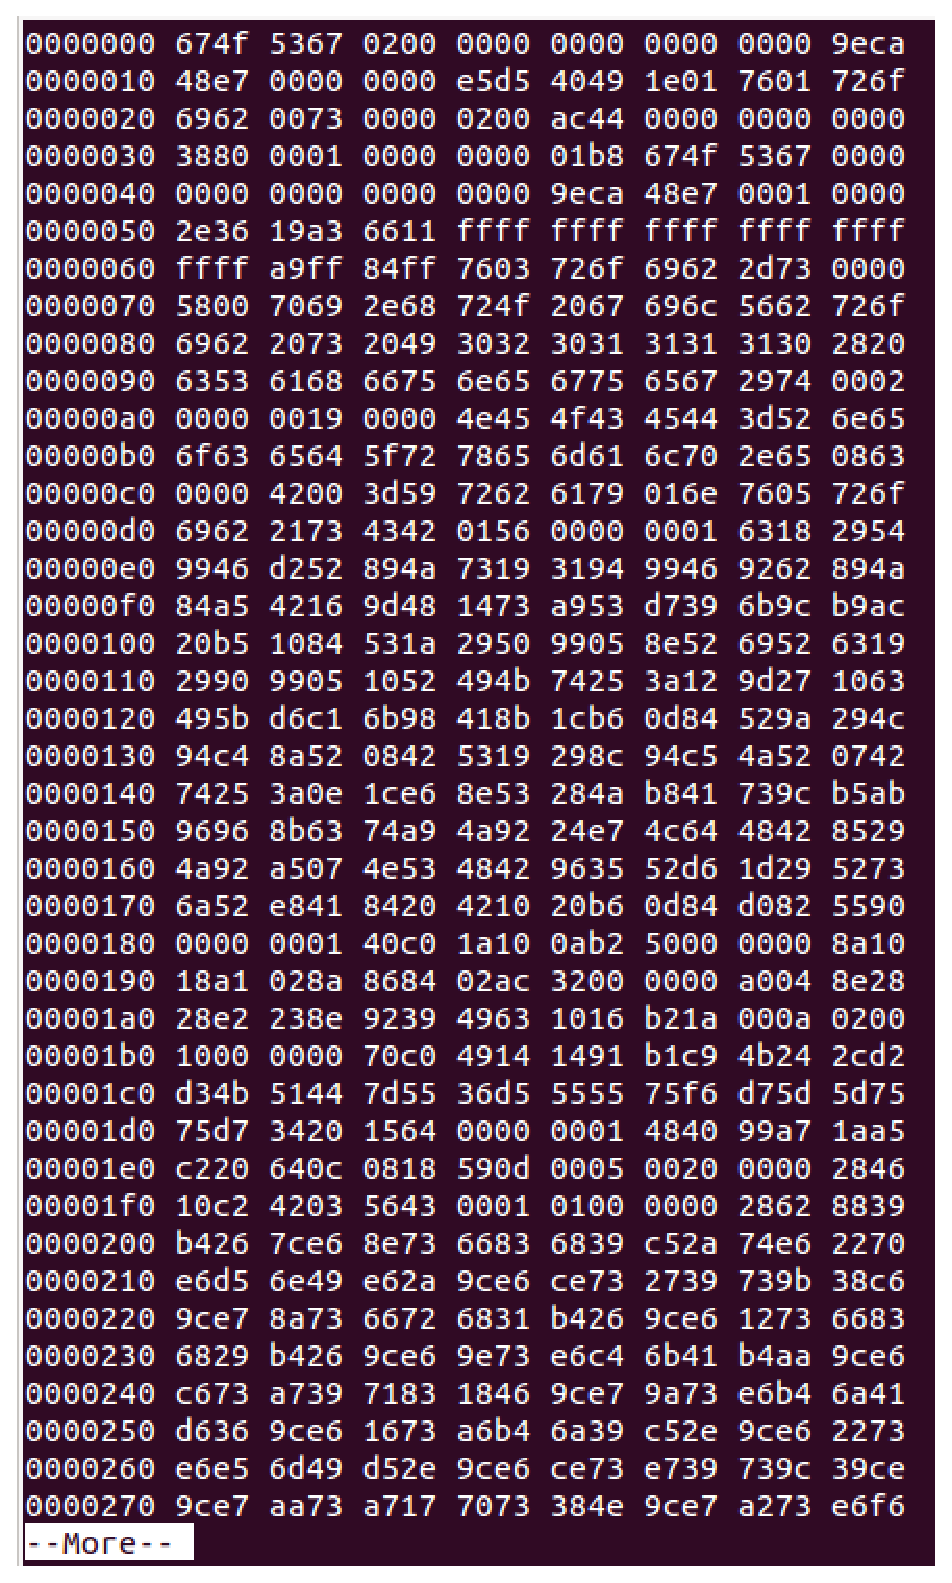
\includegraphics[keepaspectratio=true,scale=0.5]{figuras/hexdump.eps}
	\caption{Execução da ferramenta hexdump.}
	\label{hexdump}
\end{figure}

No entanto, os dados ainda ficaram muito confusos e de difícil interpretação. Após uma pesquisa verificou-se a existência de uma outra ferramenta também nativa no sistema operacional Ubuntu e voltada para os arquivos com extensão *.ogg. A ferramenta, basicamente, possui a mesma finalidade da ferramenta hexdump. A diferença está na forma com que ela apresenta os dados. Podemos verificar na Figura \ref{oggzdump} como os dados são apresentados. O comando para execução da ferramenta é dado no terminal e possui o seguinte formato: \textit{oggz-dump <file\_name>}.

 \begin{figure}[ht]
	\centering
		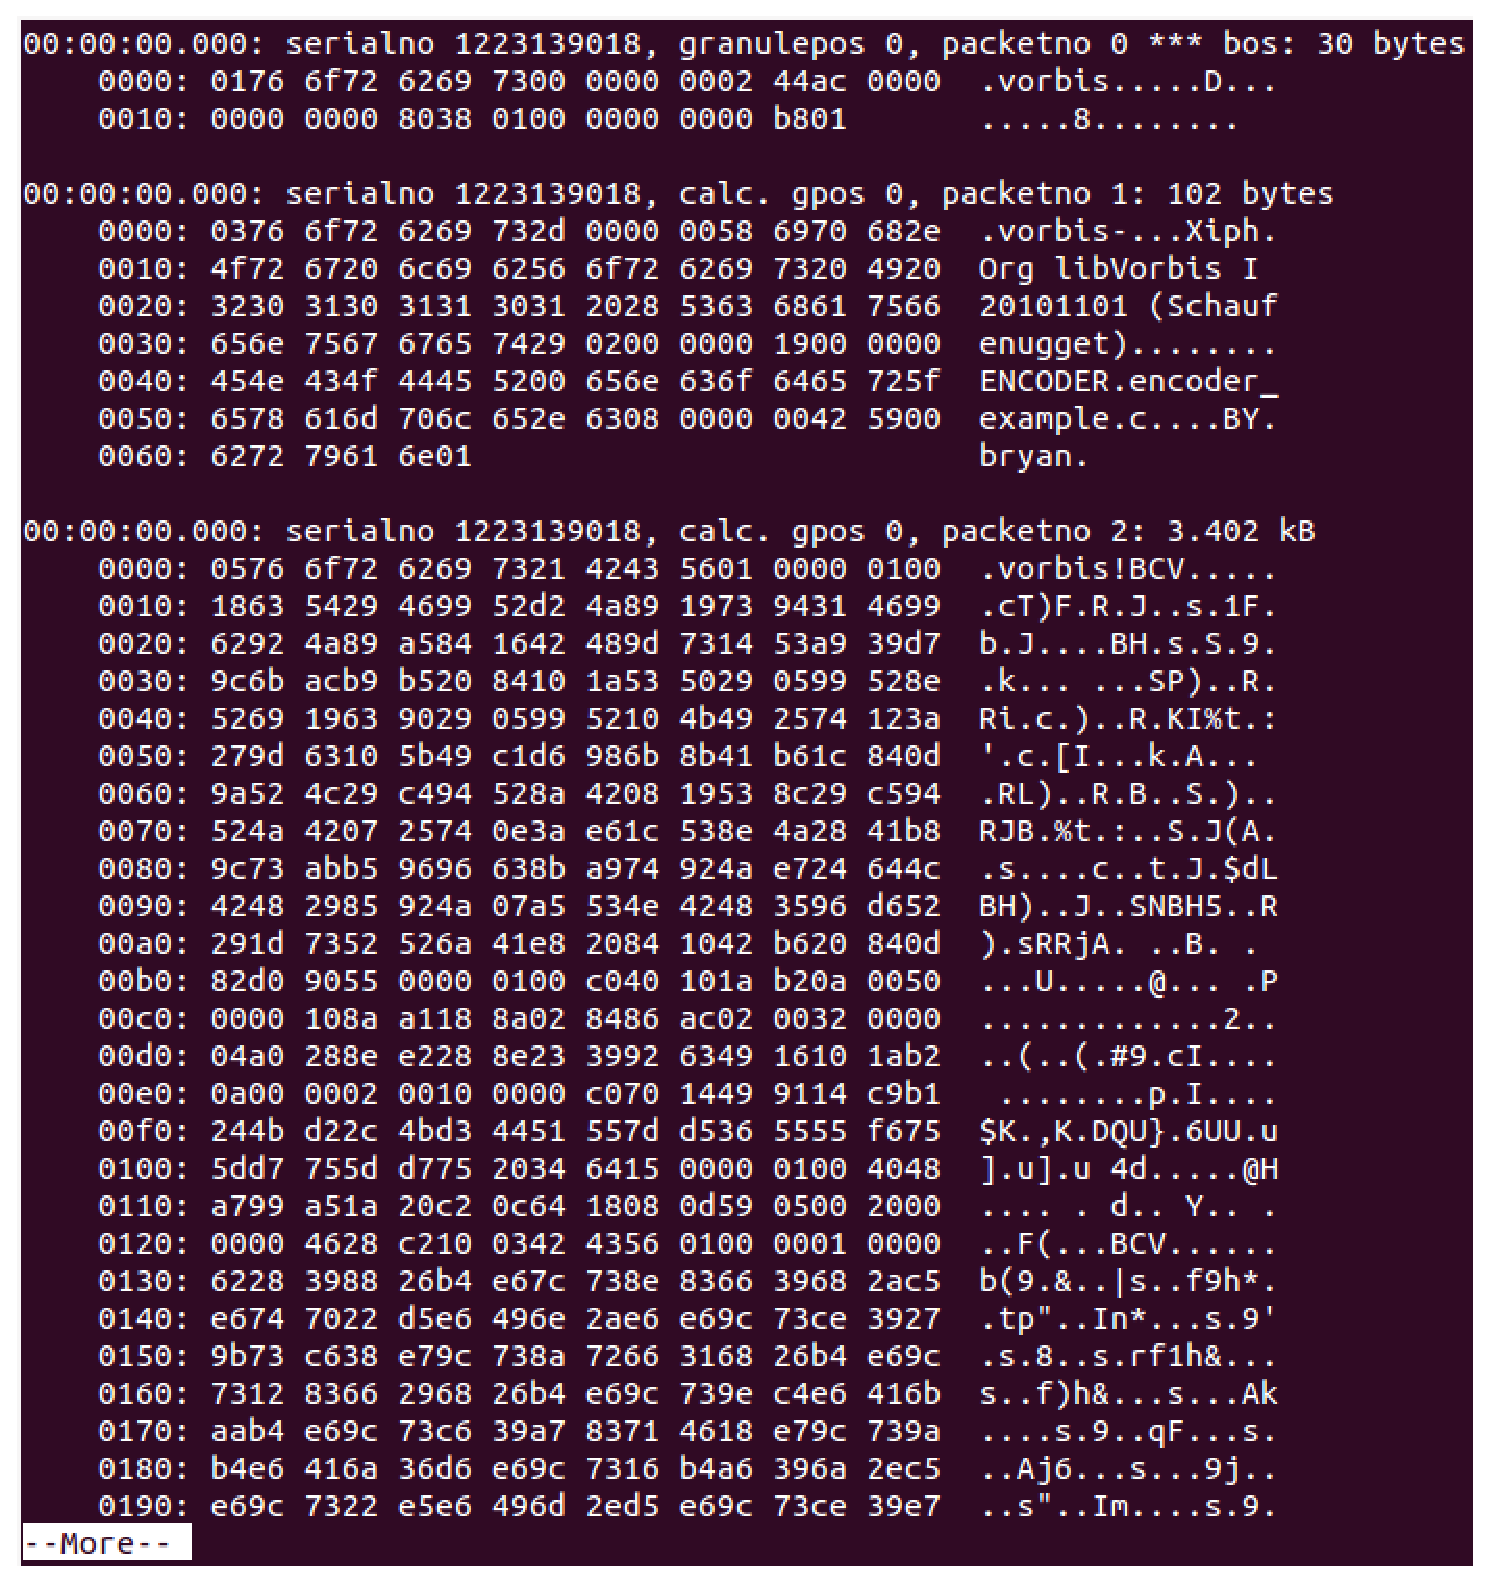
\includegraphics[keepaspectratio=true,scale=0.5]{figuras/oggz-dump.eps}
	\caption{Execução da ferramenta oggzdump.}
	\label{oggzdump}
\end{figure}

É notável a diferença e a facilidade com que a ferramenta oggz informa sobre os pacotes contidos em um arquivo *.ogg. Após o comando é possível verificar os pacotes separadamente bem como sua informações tais como número do pacote, informações de grânulo, o ``tempo'' em que aquele pacote é lido, o seu tamanho, entre outras informações. Além das informações do pacote também é possível visualizar se conteúdo e logo percebemos que os pacotes número 0, 1 e 2 são os pacotes cabeçalhos. É fácil identificar os pacotes cabeçalhos pois após o primeiro byte do pacote, os 6 bytes subsequentes contém a string ``vorbis'' onde cada byte representa uma letra.

\section{Construção do codificador}

O estudo e o processo acima foi realizado para entender a estrutura do Ogg Vorbis e onde inserir os metadados e as marcações de conteúdo validando, assim, a possibilidade do uso do formato para a solução do problema. Para dar continuidade no estudo de viabilidade do formato Ogg Vorbis, foi desenvolvido um codificador em linguagem c. Como suporte, foram utilizadas as bibliotecas \textit{logg}, \textit{lvorbis} e \textit{lvorbisenc}. Para compilar o arquivo é necessário utilizar o seguinte comando: \textit{gcc -o <nome\_para\_o\_executável> <código\_fonte> -logg -lvorbis -lvorbisenc}. Para garantir que o processo de codificação realmente funcionasse, foi utilizado outro formato no processão de codificação de um formato Ogg Vorbis. O código desenvolvido pega o conteúdo sonoro de um formato WAVE e o codifica em Ogg Vorbis, com os seus dados comprimidos. Basicamente, o PCM do formato WAVE é decodificado e posto em memória e, em seguida, os pacotes cabeçalhos do Ogg Vorbis são construídos. O PCM passa a ser inserido dentro do pacote de áudio finalizando o processo de decodificação. A ferramenta \textit{oggz-dump} foi executada no arquivo gerado e após análise, os pacotes cabeçalhos, em tese, foram codificados corretamente. Para verificar se a integridade do arquivo não foi corrompida, utilizou-se o player Sound Exchange licenciado sob a GNU General Public License e distribuído por Chris Bagwell através \cite{sox}. Este player possui uma interface de linha de comando e, ao utilizá-lo, era possível executar o som, este agora no formato Ogg, sem interrupção. O arquivo WAVE ocupava um espaço de 1.4MB em memória e após a codificação, o arquivo Ogg Vorbis ocupou apenas 86kb.


%A decisão para uso deste formato foi de rápida aceitação pois, além de ser open source, ele possui licença BSD e seu formato faz uso de compressão de dados.

\subsection{Inserção dos metadados}

Como fundamentado teoricamente no item mais acima, o arquivo *.ogg possui um pacote onde é possível inserir comentários. O \textit{comment packet} é o segundo pacote de cabeçalho da sequência de três que o Ogg Vorbis utiliza. Na Figura \ref{oggzdump} ele aparece como o pacote número 1. O próximo passo então foi inserir, comentários referentes ao arquivo de áudio. Logo, o pacote de comentários do formato Ogg Vorbis foi utilizado para inserção dos metadados e, comparando-o ao trabalho realizado \cite{herbert}, corresponde a estrutura META. Para este fim, o código desenvolvido em linguagem de programação C para a codificação foi modificado e este agora, além de pegar o conteúdo sonoro de um formato WAVE e o codificar em Ogg Vorbis com os dados comprimidos, ele também insere metadados no pacote. Para verificação da integridade do arquivo neste ponto do desenvolvimento, os mesmos passos utilizados no processo de codificação foram seguidos e as ferramentas \textit{oggz-dump} e \textit{sox} foram utilizadas.


\subsection{Construção do pacote LGMK}

Referente a estrutura LGMK \cite{herbert}, o formato *.ogg não possui suporte e se fez necessário a alteração de sua estrutura. Isso deveria ser feito, obviamente, sem que o arquivo fosse corrompido possibilitando sua execução em players comuns. Para tal finalidade, uma nova estrutura foi definida e inserida dentro do formato sem, obviamente, corrompê-lo. Foi possível codificar e também decodificar as marcações de conteúdo com integridade.

\section{Construção do decodificador}



\subsection{Decodificação dos metadados}

O metadados, uma vez codificados, precisavam ser decodificados e seu conteúdo recuperado em mémoria sem perda de dados. Para este fim, foi feito o uso da API libvorbisfile onde foi possível recuperar os metadados corretamente.


\subsection{Decodificação do pacote LGMK}

%Entender a o formato Ogg Vorbis
%Entender onde colocar os metadados
%Inserir marcações de conteúdo em um *.ogg
%Leitura de um arquivo
%Usar a API da libvorbisfile para ler e executar um audio *.ogg